\hypertarget{util_8c}{
\section{lib/util.c File Reference}
\label{util_8c}\index{lib/util.c@{lib/util.c}}
}
Useful utility functions. 

{\tt \#include \char`\"{}arrow.h\char`\"{}}\par


Include dependency graph for util.c:\nopagebreak
\begin{figure}[H]
\begin{center}
\leavevmode
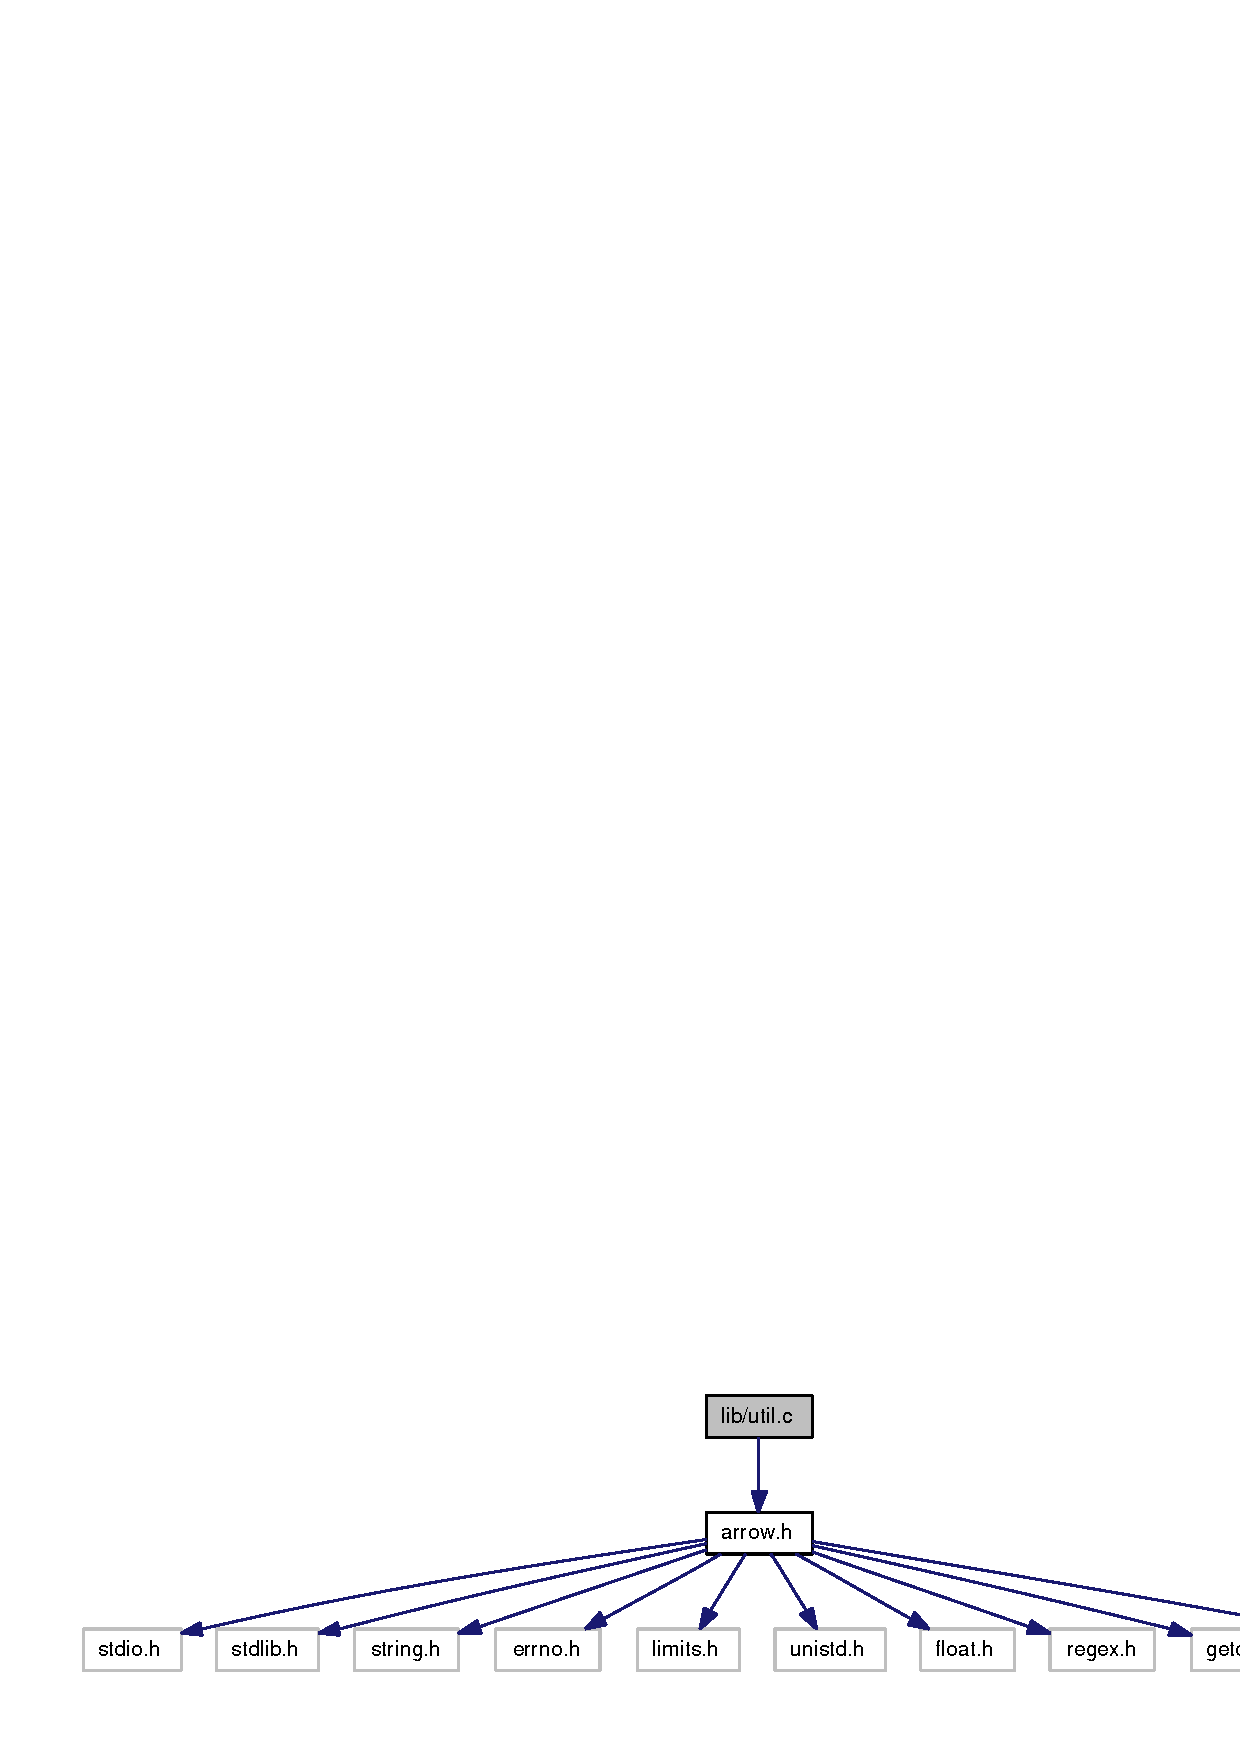
\includegraphics[width=257pt]{util_8c__incl}
\end{center}
\end{figure}
\subsection*{Functions}
\begin{CompactItemize}
\item 
int \hyperlink{util_8c_4aea68dfc908d08522baccb148251ae7}{arrow\_\-util\_\-create\_\-int\_\-array} (int size, int $\ast$$\ast$array)
\begin{CompactList}\small\item\em Creates an integer array. \item\end{CompactList}\item 
void \hyperlink{util_8c_3bd7042ebd6e97b5790a8708c91be5b4}{arrow\_\-util\_\-print\_\-error} (const char $\ast$file\_\-name, int line\_\-num, const char $\ast$message)
\begin{CompactList}\small\item\em Prints an error message to stderr with consistent formatting. \item\end{CompactList}\item 
double \hyperlink{util_8c_05b2e96c9991c51368c1f8d5a77d3ccf}{arrow\_\-util\_\-zeit} ()
\begin{CompactList}\small\item\em Used to measure timings. \item\end{CompactList}\item 
void \hyperlink{util_8c_8a9cef270a8d9d4fb22483dc986aa792}{arrow\_\-util\_\-redirect\_\-stdout\_\-to\_\-file} (const char $\ast$filename, int $\ast$old\_\-stream)
\begin{CompactList}\small\item\em Redirects STDOUT stream to a file (can be used to completely surpress output by directing to /dev/null). \item\end{CompactList}\item 
void \hyperlink{util_8c_65b9ba02b0c557fe9b15f5315a6953db}{arrow\_\-util\_\-restore\_\-stdout} (int old\_\-stream)
\begin{CompactList}\small\item\em Restores STDOUT stream that's been redirected. \item\end{CompactList}\end{CompactItemize}


\subsection{Detailed Description}
Useful utility functions. 

Useful utility functions that have general purpose throughout the library.

\begin{Desc}
\item[Author:]John LaRusic \end{Desc}


Definition in file \hyperlink{util_8c-source}{util.c}.

\subsection{Function Documentation}
\hypertarget{util_8c_4aea68dfc908d08522baccb148251ae7}{
\index{util.c@{util.c}!arrow\_\-util\_\-create\_\-int\_\-array@{arrow\_\-util\_\-create\_\-int\_\-array}}
\index{arrow\_\-util\_\-create\_\-int\_\-array@{arrow\_\-util\_\-create\_\-int\_\-array}!util.c@{util.c}}
\subsubsection{\setlength{\rightskip}{0pt plus 5cm}int arrow\_\-util\_\-create\_\-int\_\-array (int {\em size}, \/  int $\ast$$\ast$ {\em array})\hspace{0.3cm}{\tt  \mbox{[}inline\mbox{]}}}}
\label{util_8c_4aea68dfc908d08522baccb148251ae7}


Creates an integer array. 

\begin{Desc}
\item[Parameters:]
\begin{description}
\item[{\em size}]\mbox{[}in\mbox{]} size of array \item[{\em array}]\mbox{[}out\mbox{]} pointer to array that will be created \end{description}
\end{Desc}


Definition at line 15 of file util.c.

References ARROW\_\-ERROR\_\-FATAL, arrow\_\-print\_\-error, and ARROW\_\-SUCCESS.

Referenced by arrow\_\-bbssp\_\-biconnected(), arrow\_\-bintree\_\-to\_\-array(), and arrow\_\-tsp\_\-result\_\-init().\hypertarget{util_8c_3bd7042ebd6e97b5790a8708c91be5b4}{
\index{util.c@{util.c}!arrow\_\-util\_\-print\_\-error@{arrow\_\-util\_\-print\_\-error}}
\index{arrow\_\-util\_\-print\_\-error@{arrow\_\-util\_\-print\_\-error}!util.c@{util.c}}
\subsubsection{\setlength{\rightskip}{0pt plus 5cm}void arrow\_\-util\_\-print\_\-error (const char $\ast$ {\em file\_\-name}, \/  int {\em line\_\-num}, \/  const char $\ast$ {\em message})\hspace{0.3cm}{\tt  \mbox{[}inline\mbox{]}}}}
\label{util_8c_3bd7042ebd6e97b5790a8708c91be5b4}


Prints an error message to stderr with consistent formatting. 

\begin{Desc}
\item[Parameters:]
\begin{description}
\item[{\em file\_\-name}]\mbox{[}in\mbox{]} file error occured in \item[{\em line\_\-num}]\mbox{[}in\mbox{]} line number error occured at \item[{\em message}]\mbox{[}in\mbox{]} error message to write \end{description}
\end{Desc}


Definition at line 27 of file util.c.\hypertarget{util_8c_8a9cef270a8d9d4fb22483dc986aa792}{
\index{util.c@{util.c}!arrow\_\-util\_\-redirect\_\-stdout\_\-to\_\-file@{arrow\_\-util\_\-redirect\_\-stdout\_\-to\_\-file}}
\index{arrow\_\-util\_\-redirect\_\-stdout\_\-to\_\-file@{arrow\_\-util\_\-redirect\_\-stdout\_\-to\_\-file}!util.c@{util.c}}
\subsubsection{\setlength{\rightskip}{0pt plus 5cm}void arrow\_\-util\_\-redirect\_\-stdout\_\-to\_\-file (const char $\ast$ {\em filename}, \/  int $\ast$ {\em old\_\-stream})}}
\label{util_8c_8a9cef270a8d9d4fb22483dc986aa792}


Redirects STDOUT stream to a file (can be used to completely surpress output by directing to /dev/null). 

\begin{Desc}
\item[Parameters:]
\begin{description}
\item[{\em filename}]\mbox{[}in\mbox{]} name of file to direct STDOUT to \item[{\em old\_\-stream}]\mbox{[}out\mbox{]} existing file handle for STDOUT stream (necessary for restoring stream afterwards) \end{description}
\end{Desc}


Definition at line 40 of file util.c.

Referenced by main().\hypertarget{util_8c_65b9ba02b0c557fe9b15f5315a6953db}{
\index{util.c@{util.c}!arrow\_\-util\_\-restore\_\-stdout@{arrow\_\-util\_\-restore\_\-stdout}}
\index{arrow\_\-util\_\-restore\_\-stdout@{arrow\_\-util\_\-restore\_\-stdout}!util.c@{util.c}}
\subsubsection{\setlength{\rightskip}{0pt plus 5cm}void arrow\_\-util\_\-restore\_\-stdout (int {\em old\_\-stream})}}
\label{util_8c_65b9ba02b0c557fe9b15f5315a6953db}


Restores STDOUT stream that's been redirected. 

\begin{Desc}
\item[Parameters:]
\begin{description}
\item[{\em old\_\-stream}]\mbox{[}in\mbox{]} existing file handle for STDOUT stream \end{description}
\end{Desc}


Definition at line 49 of file util.c.

Referenced by main().\hypertarget{util_8c_05b2e96c9991c51368c1f8d5a77d3ccf}{
\index{util.c@{util.c}!arrow\_\-util\_\-zeit@{arrow\_\-util\_\-zeit}}
\index{arrow\_\-util\_\-zeit@{arrow\_\-util\_\-zeit}!util.c@{util.c}}
\subsubsection{\setlength{\rightskip}{0pt plus 5cm}double arrow\_\-util\_\-zeit ()\hspace{0.3cm}{\tt  \mbox{[}inline\mbox{]}}}}
\label{util_8c_05b2e96c9991c51368c1f8d5a77d3ccf}


Used to measure timings. 

\begin{Desc}
\item[Returns:]a value representing the CPU time in seconds \end{Desc}


Definition at line 34 of file util.c.

Referenced by arrow\_\-bbssp\_\-solve(), and arrow\_\-tsp\_\-exact\_\-solve().